
\documentclass[10pt,letterpaper]{article}



% Some useful packages
% math
\usepackage{amsmath}
\usepackage{amsfonts}
\usepackage{algorithm}
\usepackage[noend]{algpseudocode}
\usepackage{amssymb}
% pretty colors
\usepackage{color}
% nicer urls that break at the end of the page
\usepackage{url}
% every document needs images
\usepackage{graphicx}
\usepackage{setspace}
\usepackage{caption}
\usepackage{subcaption}


\newcommand{\e}{\mathbb E}
\newcommand{\R}{\mathbb{R}}
\newcommand\given[1][]{\:#1\vert\:}
\DeclareMathOperator*{\argmin}{arg\,min} % thin space, limits underneath in displays
\DeclareMathOperator*{\argmax}{arg\,max} % thin space, limits underneath in displays
\newcommand{\var}[1]{{\operatorname{\mathit{#1}}}}
\algdef{SE}[SUBALG]{Indent}{EndIndent}{}{\algorithmicend\ }%
\algtext*{Indent}
\algtext*{EndIndent}

\graphicspath{{./figures/}}   % where to look for images

%let's fiddle with the default margins to save some trees
%this makes the odd side margin go to the default of 1inch
\oddsidemargin 0.0in
%sets the textwidth to 6.5, which leaves 1 for the remaining right margin with 8 1/2X11inch paper
\textwidth 6.5in
% less white space, please!
\headheight 0.0in
% shift everything up
\topmargin -0.5in
\footskip .6in
% text should take up all but a 1'' margin
\textheight 9.0in

% Define some shortcuts for things I want to use.
% Use them like, for example:
% \begin{hypothesis}Lettuce causes brain damage.\end{hypothesis}
% Numbering & formatting will happen automatically.
\newtheorem{hypothesis}{Hypothesis}
\newtheorem{task}{Task}
\newtheorem{contribution}{Contribution}


% Shortcuts: allows you to use limited markup when editing/collaborating.
% \comment{This section needs to be rewritten.}
\def\ask#1{\textcolor{red}{\bf $\langle\langle$Question:\ #1$\rangle\rangle$}}
\def\comment#1{\textcolor{red}{\bf $\langle\langle$Comment:\ #1$\rangle\rangle$}}


% This imitates the Wikipedia ``Citation Needed'' text; use it as a temporary
% marker for things you need to cite.
\def\citationneeded{$^{\textcolor{blue}{\text{[citation needed]}}}$ }

% format et al.
\def\etal{\textit{et al.}}
\def\ie{\textit{i.e.}}
\def\eg{\textit{e.g.}}

\title{Attempts to exercise in Reinforcement Learning book Chapter 5}
\author{Mengliao Wang}


\begin{document}

% Generate Title Page
\maketitle


% this dumps the abstract on a front page all by itself.

\section*{Exercise 5.1: }
\label{5.1}

The last two rows are the states with hand 20 and 21, which according to the policy will stop. Thus these states will never take the risk of going bust comparing to other states, and resulting in much higher values.\\
For the most left column which means opponent shows a card ace, it indicates that opponent might have a usable ace. As we can tell from the state values, that states with a usable ace normally have higher value than the states without a usable ace, because it gives more flexibility and reduces the risk of going bust. That is also why the most font row in the upper diagram has higher values than the lower diagram.

\section*{Exercise 5.2: }
\label{5.2}


\begin{figure}[htp]
\begin{center}
  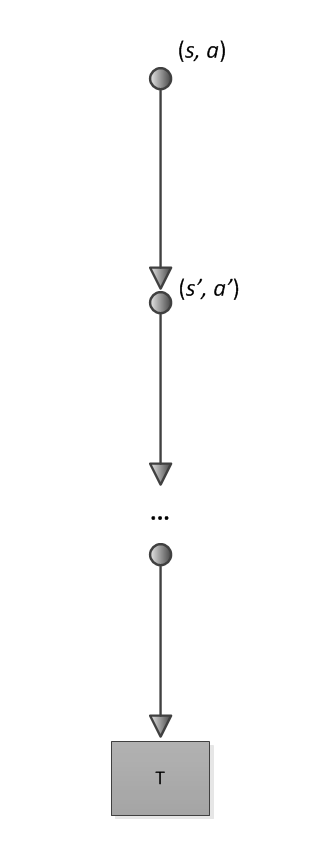
\includegraphics[scale=0.2]{backup_mc_q}

\end{center}
  \caption{The backup diagram for $q_\pi$ estimation}
  \label{fig:backup_mc_q}
\end{figure}

The backup diagram for $q_\pi$ is shown as in Figure \ref{fig:backup_mc_q}

\section*{Exercise 5.3: }
\label{5.3}

According to the definition of $q_\pi(s,a)$, we can easily have as the following analogous. Here we updated the timing for ratio $\rho$ to from $t$ to $t+1$, because the action for time $t$ is already determined.

\begin{align}
Q(s,a) &= \dfrac{\sum_{t\in \mathcal{T}(s,a)}\rho_{t+1}^{T(t)}G_t}{\sum_{t\in \mathcal{T}(s,a)}\rho_{t+1}^{T(t)}}
\end{align}

\section*{Exercise 5.4: }
\label{5.4}

The MSE increases at the beginning because the weighted estimate is bias towards $V_b$ with few training samples (with only one sample the expectation is exactly $V_b$). Here the behaviour policy is randomly stick or hit, which is very different from the target policy (stick only on a sum of 20 or 21). Thus initially the weighted estimate shows a bigger difference from the real values for target policy $V_\pi$. However as the episode number increases, estimate will converge to the expectation of $V_\pi$ instead of $V_b$, thus the MSE decreased later.

\section*{Exercise 5.5: }
\label{5.5}

Yes the variance of the estimate will still be infinite. For both method, $\e[X^2]$ can be written as: 
\begin{equation}
\e\left[\left(\sum_{k\in\mathcal{T}(s)}\prod_{t=k}^{T-1}\dfrac{\pi(A_t|S_t)}{\mu(A_t|S_t)}G_k\right)^2\right]
\end{equation}

For first-visit method we will define $\mathcal{T}(s)$ to be the first time we observe state s, which is obviously time step 0, then we have the same expression as in the book. For every-visit method, we will define $\mathcal{T}(s)$ to be the all the times we could observe state s, e.g. 0, 1, 2, .... Thus for every-visit method it is:

\begin{equation}
\e\left[\left(\sum_{k=0}^{T-1}\prod_{t=k}^{T-1}\dfrac{\pi(A_t|S_t)}{\mu(A_t|S_t)}G_k\right)^2\right]
\end{equation}

Follow the same calculation as shown in the book can find that $\e\left[\left(\prod_{t=k}^{T-1}\dfrac{\pi(A_t|S_t)}{\mu(A_t|S_t)}G_k\right)^2\right], \forall k <= T-1$ is the same as $\e\left[\left(\prod_{t=0}^{T-1}\dfrac{\pi(A_t|S_t)}{\mu(A_t|S_t)}G_0\right)^2\right]$. Thus obviously the whole expectation Expression (3) is still be infinite.


\section*{Exercise 5.6: }
\label{5.6}

To make the algorithm for first-visit method, we would need to hold the updated $Q(S_t,A_t)$ in a placeholder $H(S_t,A_t)$, and keep overwriting $H(S_t,A_t)$ during the for loop, so eventually $H(S_t, A_t)$ will only hold the values for the first time visit of $(S_t, A_t)$. Then we assign it to $Q(S_t, A_t)$ outside of the for loop. See the modified algorithm below:

\begin{algorithmic}
\State Initialize, for all $s\sin \mathcal{S}, a\in \mathcal{A}(s)$:
\Indent
\State $Q(s,a) \gets$ arbitrary
\State $H(s,a) \gets Q(s,a)$
\State $C(s,a) \gets 0$ 
\State $\mu(a\given s) \gets$ an arbitrary soft behavior policy
\State $\pi(a\given s) \gets$ an arbitrary target policy
\EndIndent
\Repeat
\State Generate an episode using $\mu$
\Indent
\State $S_0,A_0,R_1,...,S_{T-1},A_{T-1},R_T,S_T$
\EndIndent
\State $G \gets 0$
\State $W \gets 1$
\For {$t=T-1, T-2,...$ down to 0:}
\State $G \gets \gamma G + R_{t+1}$
\State $C(S_t, A_t) \gets C(S_t, A_t) + W$
\State $H(S_t, A_t) \gets Q(S_t, A_t) + \dfrac{W}{C(S_t,A_t)}[G-Q(S_t, A_t)]$
\State $W \gets W\dfrac{\pi(A_t\given S_t)}{\mu(A_t\given S_t)}$
\If {$W=0$:}
\State ExistForLoop
\EndIf
\EndFor
\For {Each unique pair $S_t, A_t$ appeared in the episode:}
\State $Q(S_t, A_t) \gets H(S_t, A_t)$
\EndFor
\Until{$1=1$}
\end{algorithmic}


\section*{Exercise 5.7: }
\label{5.7}

According to 5.6 we have:

\begin{align*}
V_{n+1}&= \dfrac{\sum_{k=1}^n W_k G_k}{\sum_{k=1}^n W_k} \\
&=\dfrac{\sum_{k=1}^{n-1}W_kG_k + W_nG_n}{C_n} \\
&=\dfrac{\sum_{k=1}^{n-1}W_k}{C_n}\dfrac{\sum_{k=1}^{n-1}W_kG_k}{\sum_{k=1}^{n-1}W_k} + \dfrac{W_nG_n}{C_n} \\
&=\dfrac{C_n-W_n}{C_n}V_n + \dfrac{W_nG_n}{C_n} \\
&=V_n + \dfrac{W_n}{C_n}\left[G_n-V_n\right]
\end{align*}


\section*{Exercise 5.8: }
\label{5.8}
\begin{figure}
   \centering
    \begin{subfigure}[b]{0.5\textwidth}
        \centering
        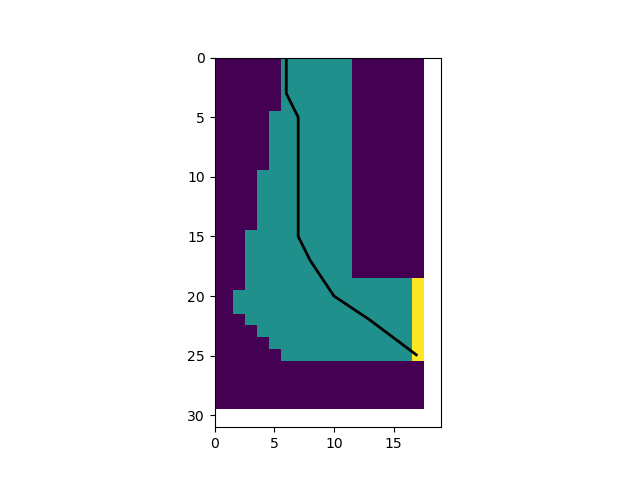
\includegraphics[scale=0.4]{RaceTrace_50}
        \caption{Results after training with 50 episodes}
    \end{subfigure}%
~
    \begin{subfigure}[b]{0.5\textwidth}
        \centering
        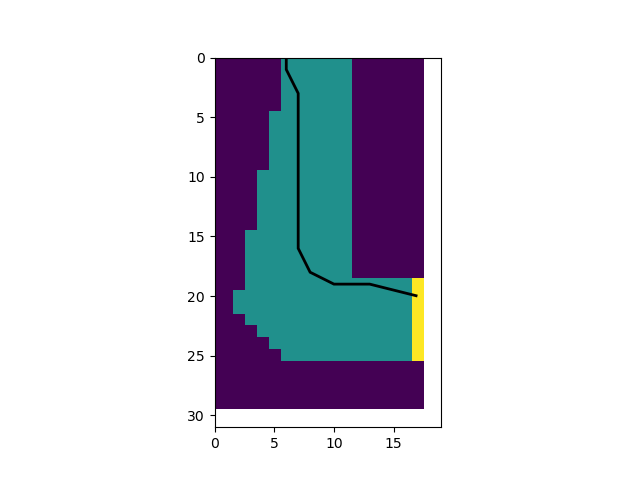
\includegraphics[scale=0.4]{RaceTrace_200}
        \caption{Results after training with 200 episodes}
    \end{subfigure}%

    \begin{subfigure}[b]{0.5\textwidth}
        \centering
        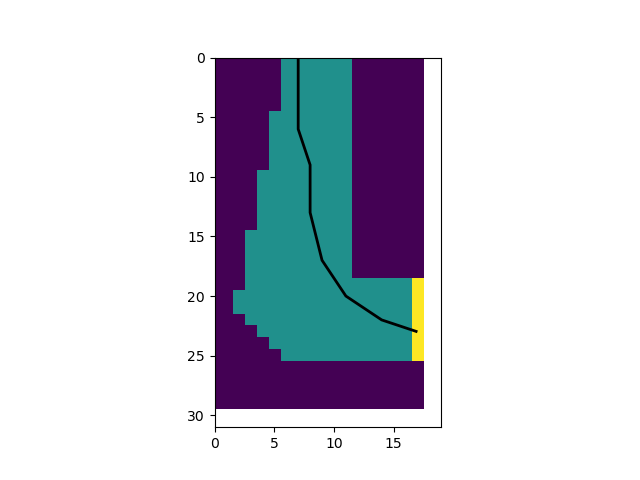
\includegraphics[scale=0.4]{RaceTrace_1000}
        \caption{Results after training with 1000 episodes}
    \end{subfigure}%
~
    \begin{subfigure}[b]{0.5\textwidth}
        \centering
        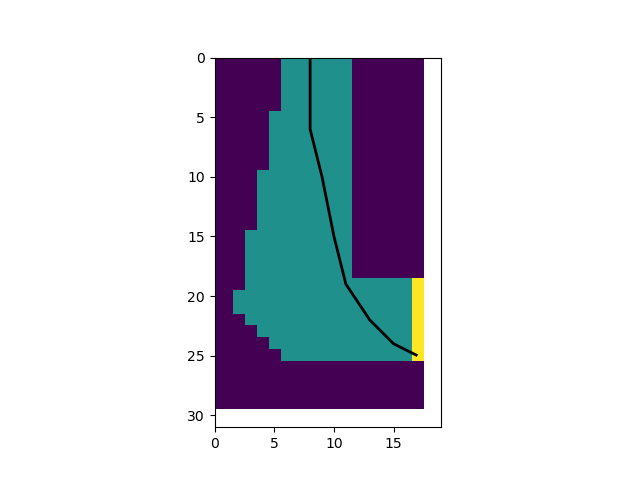
\includegraphics[scale=0.4]{RaceTrace_10000}
        \caption{Results after training with 10000 episodes}
    \end{subfigure}
    \caption{RaceTrack results after training with 50, 200, 1000, 10000 episodes}
  \label{fig:race_results}
\end{figure}

Program attached. Here are the results after learing 50, 200, 1000, 10000 episodes in Figure \ref{fig:race_results}. The green area is the track, and the yellow line is the destination.


\section*{Exercise 5.9: }
\label{5.9}

 
The algorithm would be:

\begin{algorithmic}
\State Initialize, for all $s\sin \mathcal{S}, a\in \mathcal{A}(s)$:
\Indent
\State $Q(s,a) \gets$ arbitrary
\State $C(s,a) \gets 0$ 
\State $\pi(a\given s) \gets$ a deterministic policy that is greedy with respect to Q
\EndIndent
\Repeat
\State Generate an episode using any soft policy $\mu$
\Indent
\State $S_0,A_0,R_1,...,S_{T-1},A_{T-1},R_T,S_T$
\EndIndent
\State $G\gets 0$
\For {$t=T-1, T-2,...$ down to 0:}
\State $\rho \gets 1$
\State $\bar{G}\gets 0$
\State $W \gets 0$
\For {$k=t+1, t+2,...$ until $T-1$:}
\State $\bar{G}\gets \bar{G} + R_k$
\State $\rho \gets \rho\dfrac{\pi(A_k\given S_k)}{\mu(A_k\given S_k)}$
\State $W \gets W +(1-\gamma)\gamma^{k-t-1}\rho$
\State $G\gets G + W\bar{G}$
\EndFor
\State $W \gets W + \gamma^{T-t-1}\rho$
\State $G\gets G + W\bar{G}$
\State $C(S_t, A_t) = C(S_t, A_t) + W$
\State $Q(S_t, A_t) \gets Q(S_t, A_t) + \dfrac{W}{C(S_t,A_t)}[G-Q(S_t, A_t)]$
\State $\pi(S_t) \gets \argmax_a Q(S_t, a)$
\If {$A_t\neq \pi(S_t)$:}
\State ExistForLoop
\EndIf
\EndFor
\Until{$1=1$}
\end{algorithmic}


\clearpage

\end{document}
